\chapter{Реформы Мария, которые были}
\begin{remark}
	Внимание: в тексте ниже я ни в чем себе не отказываю, разговариваю матом и препарирую оппонента без анестезии. Если вас такое смущает, то немедленно прекратите чтение. Спасибо.
\end{remark}
Итак, Марианская реформа. В интернете, в журнале Варспот есть одна примечательная статья за авторством Алексея Козленко. Где данный автор решил огорошить нас охуительным тезисом о том, что никакой реформы не было, политрук лжет и вообще как-то всё само собой произошло. Написана она почти 5 лет назад, в ноябре 2015 года, и несмотря на свою кетаминовую бредовость продолжает находить своего читателя. В меня её кидали как минимум раз двадцать, последний раз - вчера вечером. И если первым юным натуралистам я просто на пальцах пояснял чому статья — набор хуеты, то последний раз вполне адекватный в других вопросах человек уже как аксиому вывел что «реформы не было, томушта так на Варспоте написано». Тоесть мифотворчество пустило корни, и на высер ссылаются практически как на Википедию. Поэтому я решил что хватит это терпеть и пора выходить на поле боя. Иначе наши дети так и вырастут идиотами, которым никто не объяснил что не всё что написано в интернет-журнале не является кликбейтовой ебаниной. Ну и дабы как-то компенсировать моральный вред, причиненный автору, я \href{https://warspot.ru/4023-mif-drevnego-rima-voennye-reformy-mariya}{дам ссылку}  на его статью, а также процитирую её тут целиком, благо она относительно небольшая.


Приступим.


\textit{
	В ходе дискуссий на военно-исторических форумах автору неоднократно приходилось сталкиваться с апелляцией участников к «реформе Мария». Этот же концепт присутствует в популярной и даже специальной литературе, причём авторы далеко не всегда берут на себя труд объяснить его содержание. Как среди историков-любителей, так и среди профессионалов преобладает отношение к «реформе Мария» как общеизвестному факту, не требующему специальных доказательств. На самом деле военная реформа, связываемая с именем Мария, является искусственным концептом, объединяющим явления и процессы, развивавшиеся на протяжении длительного времени и зачастую вне всякой связи с именем этого военачальника и политического деятеля.}

\textit{Широкая околоисторическая общественность связывает "реформы Мария" с начальной стадией профессионализации римской армии. Персональная заслуга в этом процессе обычно приписывается самому Марию, который выступает в качестве создателя армии нового типа. Среди осуществлённых им военных нововведений обычно перечисляют следующие:}
%\textit{
	\begin{itemize}
		\item переход к комплектованию армии из малообеспеченных слоёв пролетариата;
		\item  организация постоянных легионов, размещавшихся на территории завоёванных провинций
		\item  изменения в организационной структуре легионов, упразднение прежнего деления на манипулы, введение когорт в качестве новых штатных единиц; исчезновение деления легионеров на гастатов, принципов и триариев
		\item введение единообразного снабжения солдат. Проанализируем каждую из перечисленных реформ на предмет их соответствия деятельности Мария.
	\end{itemize}
%}




Стартовый тезис охуительностью не блещет, скромненько так, без огонька, хотя пассажи про «более внимательное рассмотрение» и «на самом деле» уже должны насторожить. Тут просто отмечу что «реформа Мария», классически, это именно реформа Мария, а не какие-то протекающие веками процессы. Процессы протекают, Марий реформирует армию и делает многое новой нормой, ЛИЧНО, обращаю внимание. Это никак друг другу не мешает. Но дальше мы убедимся, что автор за своим «не всё так однозначно» скрывает именно что «всё однозначно, Марий нихера нового не ввел», так что пусть вас приглаженный стиль не смущает.

Едем дальше. 

\section{Первый охуительный тезис}
\textbf{\textit{Комплектование}}
\textit{Из всех «реформ Мария» важнейшие последствия имеет переход к военному набору пролетариев. Информация о предпринятом Марием наборе бедноты базируется на прямых указаниях Саллюстия, (Sall. Jug., 86, 2), Геллия (Gell., XVI, 10, 14), Плутарха (Plut. Mar., 9), Валерия Максима (Val. Max. II, 3, 1), Флора (Flor., I, 36, 13). Саллюстий и Плутарх датируют это мероприятие первым консульством Мария в 107 г., Геллий хотя и принимает ту же дату, но упоминает о традиции, датировавшей это мероприятие 105 г. Чтобы выяснить, какие мероприятия осуществил Марий, по каким причинам и с какими последствиями, следует кратко остановиться на правилах набора в римскую армию.}


\textit{Согласно конституции Сервия Туллия, римский народ делился на пять имущественных разрядов, каждый из которых выставлял определённое количество воинов. За пределами пяти разрядов (соответственно выражению источников «infra classem») находились неимущие граждане, не обладавшие достаточным состоянием, чтобы самостоятельно приобрести оружие. Ливий сообщает, что к числу пролетариев относились те, чьё имущество оценивалось менее чем в 11 000 ассов, т.е. минимальная планка для пятого имущественного разряда. Пролетариев призывали только при объявлении чрезвычайного положения: во время войны с Пирром в 281 г. до н.э., (Gell., XVI, 10, 1; Oros., IV, 1, 3; Aug., De civ. Dei, III, 17), после поражения у Тразименского озера и при Каннах (Liv., XXII, 11, 8; XXII, 59). При обычных обстоятельствах они служили во флоте (Liv., XXII, 11, 8; Polyb., VI, 19, 3). Такое положение сохранялось вплоть до II Пунической войны.}


\textit{Полибий, описывая римскую армию около 160 г. до н.э., сообщает, что минимальным имущественным цензом для службы в армии является сумма в 4000 римских ассов (Polyb., VI, 19, 2). Эта сумма в 2,5 раза ниже той, которую указывает Ливий. Расхождение цифр исследователи считают результатом понижения имущественной планки для военнообязанных граждан V разряда. Э. Габба предложил датировать это мероприятие началом II Пунической войны. Он указал на данные Ливия о призыве пролетариев на военную службу в 217 и 214 гг. до н.э. и на неожиданное отсутствие этих данных для последующего времени. Ливий сообщает о призыве вольноотпущенников, об освобождении рабов, но ничего не говорит о римских пролетариях. Это умалчивание объясняется понижением имущественной планки для военного набора, что позволяло сенату рекрутировать верхушку пролетариата без объявления чрезвычайного положения. Скорее всего, пролетарии служили легковооружёнными велитами, впервые появившимися на кампанском театре военных действий в 212 г. (Val. Max. II, 3, 3).}


\textit{Сумма в 4000 ассов также не является окончательной. Цицерон в середине I в. до н.э. утверждает, что граница между гражданами V имущественного класса и пролетариями проходит по сумме в 1500 ассов (Cic. De Rep., II, 40; Gell., XVI, 10, 10) 3). Хотя Цицерон приписывает подобное положение вещей эпохе Сервия Туллия, очевидно, что уменьшение указанной Полибием суммы ценза в 4000 римских ассов произошло только во второй половине II в. до н.э. Чрезвычайно заманчивым представляется связать это мероприятие с действиями Мария, но наиболее распространённой к настоящему моменту является другая гипотеза. Э. Габба предложил датировать это событие 123 г. и связать его с военным законодательством Гая Гракха. Привлечение пролетариев к военной службе дополнялось законами о вооружении рекрутов за государственный счёт и о минимальном призывном возрасте в 17 лет, что должно было защитить новый класс военнообязанных от злоупотреблений (Plut. Grach., 26, 5). В 109 г. некоторые из этих законов оказались отменены (Asc. In Corn. P.54, 25), однако нижняя планка призывного разряда так и осталась на уровне 1500 ассов.}


\textit{Данное предположение кажется убедительным и заслуживает большего доверия, чем гипотеза, приписывающая авторство этого нововведения Марию. Все источники, находящиеся в нашем распоряжении, отмечают необычный характер предпринятого Марием набора. Прежде всего, оговоримся, что ни в 107 г., ни в два года спустя Марий не набирал новой армии. Он получал командование над действующей армией, набранной в первом случае Метеллом, во втором случае Рутилием Руфом. Марий набирал лишь пополнения, необходимые, чтобы восполнить потери. Их численность для армии из двух легионов вряд ли превышала 3000 человек. Сенат, по словам Саллюстия, охотно предоставил консулу возможность провести набор, втайне надеясь, что эта непопулярная мера ослабит его авторитет среди простонародья. Марий, раскусив этот замысел, не стал прибегать к обычному набору и навербовал себе добровольцев из числа социальных низов. Тем самым он сохранил поддержку народа и получил необходимые подкрепления (Sall. Jug., 86). Следует отметить, что Марий не создавал своими действиями исторического прецедента. Аналогичным образом ранее поступали и другие римские военачальники, находившиеся в сложных отношениях с Сенатом (App. Iber., 38).}

так, краткая суть скринов выше: «до Мария ценз снижался и так, а он его просто занизил до нуля, расходитесь, тут не на что смотреть». Тоесть автор сам же озвучивает ОСНОВНУЮ фишку того что продавил и принял как стандарт ЛИЧНО Марий, но в силу общей бестолковости в упор этого не видит, что очень смешно.


Поясняю на пальцах. ДО Мария в армию набирались люди по цензу, минимальный ценз был в 1500 ассов. Нихуя не помню сколько это, но это мелкие собственники земли, по большей части. ПОСЛЕ Мария стандартом стал набор пролетариев без ценза вообще. Добровольного набора, обращаю внимание. Разница очевидна любому нормальному человеку, в первом случае мы ПРИЗЫВАЕМ на действующую службу резервистов ПО ТРИБАМ (призывным округам), во втором случае мы открываем рекрутский набор КОГО УГОДНО вообще, и гребем мобрезерв. Сосредоточившись на безземельном люмпен-пролетариате (городской бедноте), у которого НЕТ СОБСТВЕННОСТИ, а значит он может служить 510 лет и не испытывать по этому поводу никаких проблем. Так как пока он служит — его кормят и платят жалование, а в конце обещан домик в деревне, предел мечтаний люмпенов и то что нахуй не нужно земельным крестьянам, из которых формировались легионы ДО Мария.


\textbf{Вывод: Тезис несостоятелен, автор виляет и накидывает ссылок на источники, но даже из его собственного текста очевидно что он пиздит.}

\section{Второй охуительный тезис}
\textbf{\textit{Организация постоянных легионов, размещавшихся в завоёванных провинциях}}

\textit{Основной частью римской армии был легион. В VI–III вв. до н.э. легионы обычно создавались для одной кампании и включали воинов одного набора. По окончании летней кампании легион распускался, а весной набирался заново. В обычных условиях армия состояла из четырёх легионов, которыми командовали два консула. При необходимости вести длительные войны старые легионы не распускали, а из новобранцев весеннего призыва формировали дополнительные легионы. Так, во время II Пунической войны римская армия насчитывала 28 легионов. После 200 г. до н.э. она обычно состояла из 8 легионов, иногда меньше, иногда больше. С увеличением числа провинций количество легионов возрастало. От 2 до 4 легионов постоянно находилось в Испании, 2 в Цизальпинской Галлии, 2 в Македонии и Иллирии. В начале I в. до н.э. к числу провинций прибавились Африка, Киликия, Вифиния, а количество размещавшихся на их территории легионов достигло 14.}


\textit{Единственное отличие этой практики от применявшейся в эпоху империи состояло в длительности военной службы солдат. Хотя любой римский гражданин был обязан служить в армии на протяжении 20 лет (Polyb., VI, 19, 4), на деле срок военной службы обычно составлял максимум 4–6 лет, после чего солдат старого призыва демобилизовывали и заменяли новым пополнением. Дольше других служили добровольцы, избиравшие карьеру профессиональных военных. Известным примером является Спурий Лигустин, который к достижению 50-летнего возраста служил 22 года в должности солдата и центуриона (Liv., XLII, 34). C ростом милитаризма Римской республики количество ветеранов в армии возрастало. Если в начале II в. до н.э. военная служба охватывала примерно треть взрослого населения Республики, то к середине следующего столетия служила уже половина мужчин.}


\textit{Таким образом, в римской армии в ходе II–I вв. до н.э. существовала отчётливая тенденция к профессионализации. Легионы постепенно превращались в постоянные боевые единицы, в их рядах служили воины, большей частью имевшие опыт военных походов. Этот процесс имел сложный системный характер и ни в коей мере не являлся результатом деятельности одного человека.}

Второй тезис, о профессионализации армии, доказательством которого автор почему-то считает количество легионов, которое постоянно росло. И никак его не поясняя. Тезис мутный как утренняя блевота первого января. А соль вообще в другом. Профессионализация армии это создание «людей войны», оружия, посланников смерти, молящихся чтоб начался поход. Куда угодно, против кого угодно. Что напрямую вытекает из первого пункта: нужно было пушечное мясо которому нечего терять кроме своих оков. И Марий его дал. Римляне к концу первого века УСТАЛИ воевать, они перестали заваливать противника массой качественной, дешевой и хорошо мотивированной пехоты, а по другому воевать просто не умели. И поэтому начали проебывать раз за разом. Та же Югуртинская война это очень ясно показала, что крестьянам есть что терять, и они не хотят умирать в Африке непонятно за что. Поэтому как военные они очень хуево справлялись с задачами. Собственно, Рим начал испытывать классические проблемы ПРИЗЫВНОЙ АРМИИ, когда людей призвали а нахуя им эта война - объяснить забыли.


Из забавного: автор там выдает охуительное про то что римляне были обязаны служить 20 лет, но по факту служили 4-6 лет, ссылаясь на Полибия. Я не поленился и нашел о чем там Полибий говорит по ссылке:

\begin{figure}[h!tb]
	\centering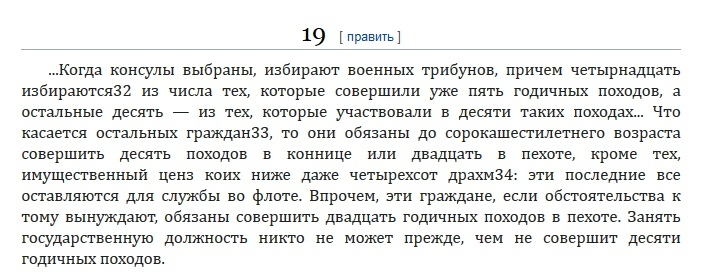
\includegraphics[scale=0.6]{Mariy/1601698942180418339.png}
	%	\label{fig:scipion} % Unique label used for referencing the figure in-text
	%	%\addcontentsline{toc}{figure}{Figure \ref{fig:placeholder}} % Uncomment to add the figure to the table of contents
	\caption{Слова Полибия}
\end{figure}

Это ценз на магистратов, блядь. На госслужащих. Тоесть хочешь участвовать в политике - иди в армию, ходи в походы. Не хочешь - копай грядки. Кто у вас землю копать будет, если все по двадцать лет в походы ходят? Второй тезис вообще крайне охуителен, настолько, что даже какой-нибудь мутный пруф к нему приложить забыли:

\textit{C ростом милитаризма Римской республики количество ветеранов в армии возрастало. Если в начале II в. до н.э. военная служба охватывала примерно треть взрослого населения Республики, то к середине следующего столетия служила уже половина мужчин.}

ОТКУДА ТЫ ЭТО ВЗЯЛ, ЕПТЕТЬ? Как ты себе представляешь вообще жизнь Республики второго века (держава на трех континентах с миллионным населением) где служат половина мужчин? Или может имеется ввиду что они в поход по разу сходили? Ну дык это как раз довод в пользу того что армия — ебучее ополчение, через которое прогоняют каждого второго. А главное: это же вообще никак не соотносится с основным тезисом. Автор просто не отдупляет что такое «профессионализация», о чем тут можно говорить?


\textbf{Вывод: создание бенефициаров войны, особой военной касты со своими социальными лифтами, это и есть «профессионализация армии» фром Марий. А то что несет этот замечательный человек — просто вода ебаная, рассчитанная на обывателя.
}

\section{Третий охуительный тезис}

\textbf{\textit{Изменения в организационной структуре легионов}}

\textit{Вопреки распространённому мнению, когорты в римской армии появились задолго до Мария. Слово «когорта» имеет древнее происхождение и, возможно, связано со способом набора войска, практиковавшимся у италиков. Когорта неоднократно упоминается в качестве элемента строя как италийских противников Рима (Liv., II, 14, 3; X, 40, 6), так и самих римлян (Liv., II, 11, 8; IV, 27, 10). Анализ этого термина показывает, что в источниках под ним подразумеваются отдельные отряды, выделенные из массы войска для решения особой задачи. Когорты в испанской армии Сципиона, как правило, включали 3 манипулы пехоты, 3 илы конницы и легковооружённых велитов (Polyb., XI, 21, 1; 33, 1). При этом когорта оставалась временным образованием, распускавшимся по выполнении возложенной на неё задачи. Особо следует отметить отсутствие у когорт того периода собственного командира и знамени.}


\textit{Основной боевой единицей римской армии являлась центурия. У каждой центурии был свой командир и своё знамя. По центуриям римская армия выстраивалась на поле боя, располагалась в лагере, получала снаряжение и продовольствие. Манипула являлась объединением двух центурий. Командовал манипулой старший центурион, у манипулы имелась особая роль в боевом построении. Подобный порядок, сложившийся ещё в эпоху классической Республики, сохранялся до конца античности. Идея об упразднении Марием манипулярного порядка и замены его построением по когортам не выдерживает критики. С одной стороны, как письменные тексты, так и эпиграфические источники свидетельствуют о сохранении деления на манипулы и центурии в течение I в. до н.э. – III в. н.э. Те же данные свидетельствуют о сохранении прежних наименований гастатов, принципов, триариев (Caes. BC., I, 41; 44; [Caes] Afr., 83). С другой стороны, никаких тактических изменений в это время также не происходило, т.к. на поле боя войска, как и раньше, продолжали выстраиваться по центуриям.}


\begin{figure}[h!tb]
	\centering
\includegraphics[scale=0.6]{Mariy/16016990541294431.png}
	%	\label{fig:scipion} % Unique label used for referencing the figure in-text
	%	%\addcontentsline{toc}{figure}{Figure \ref{fig:placeholder}} % Uncomment to add the figure to the table of contents
	\caption{Я так больше не могу, а ведь на это реально кто-то ссылается}
\end{figure}



Итак, я спокоен, продолжим.


Поясняю разницу между центурией и когортой. Центурия это ОРГАНИЗАЦИОННАЯ ЕДИНИЦА. Организационная. Это подразделение численностью человек 60. Две центурии сводились в манипулу. Тоесть, на наши деньги, роту. Численностью уже 120 человек. Их в легионе, по штатному расписанию, было 30 штук, тоесть 60 центурий. Окей. А теперь внимание, в чем смысл ввода в эксплуатацию когорт? Когорта это 3 манипулы, сведенные в одно подразделение, численностью ~360 человек. И это, на наши деньги, уже полноценный батальон. Со своим собственным обозом, штабом и всей хуйней. Это уже не организационная а боевая единица, которая была способна действовать как в составе легиона, так и автономно от основных сил. Тогда как ДО Марианской реформы, если не вспоминать про Сципиона-Эмилиана, легион ВСЕГДА действовал единым кулаком, томушта просто не мог по другому. Все эти нагугленные автором сведЕния отдельных манипул в оперативные группы — просто разовые вынужденные акции, когда приходится часть легиона вырывать с мясом и отправлять на сольный квест. И это автором выдается за то что «когорты уже были, поэтому хули вы тут развели, Марий ничего нового не придумал». Хотя любому военному человеку, который в армии был, очевидно в чем разница между ротой и батальоном. Рота это тактическая единица. А батальон - единица оперативная, внятный инструмент войны, вполне комфортно себя чувствующий даже в полной автономке.

\begin{figure}[h!tb]
	\centering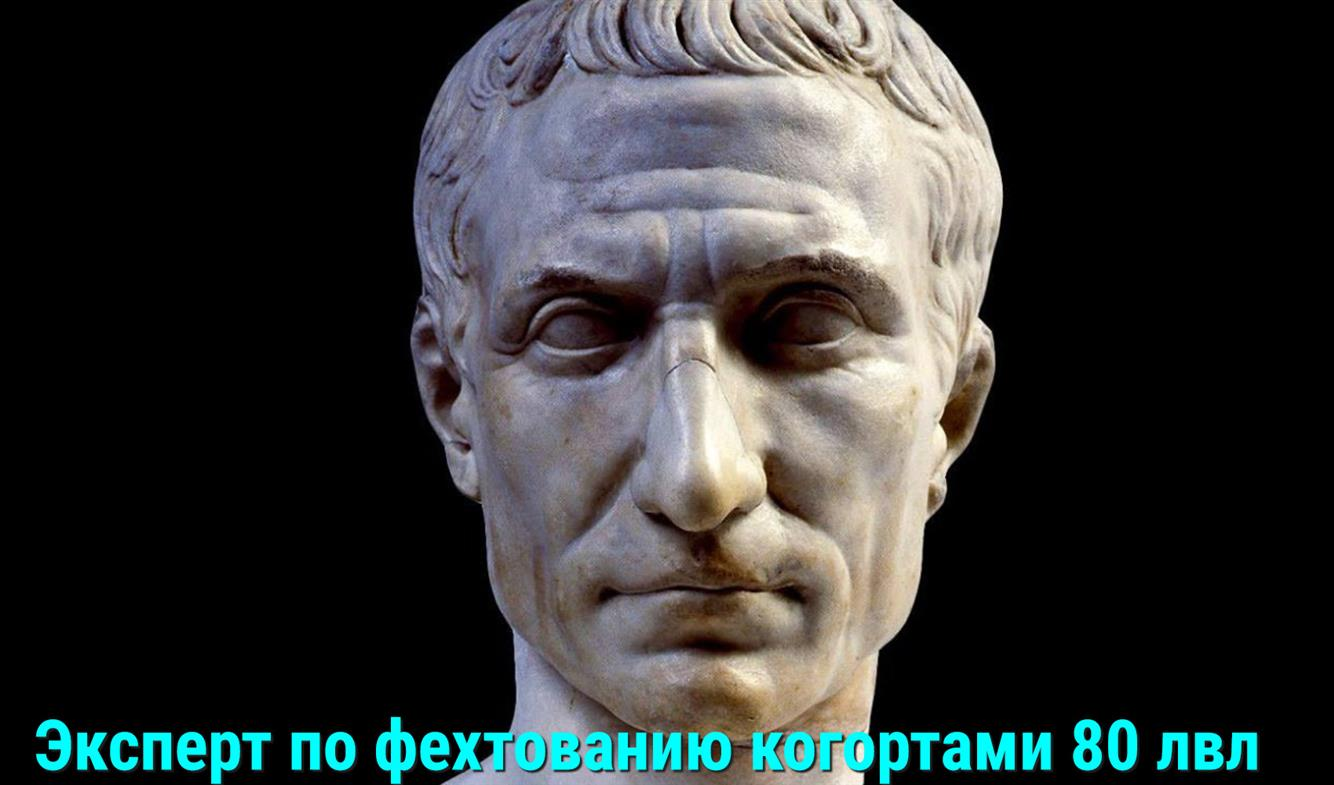
\includegraphics[scale=0.35]{Mariy/1601699074162111731.png}
	%	\label{fig:scipion} % Unique label used for referencing the figure in-text
	%	%\addcontentsline{toc}{figure}{Figure \ref{fig:placeholder}} % Uncomment to add the figure to the table of contents
	%\caption{Я так больше не могу, а ведь на это реально кто-то ссылается}
\end{figure}

Поэтому легион ДО Мария воевал целиком, он строился в пехотную фалангу (ну или по манипулярной схеме, если вы считаете что она работала) и, как единый организм, действовал на поле боя. Легион ПОСЛЕ Мария это десять батальонов, способных действовать как в составе единого легиона, так и автономно. Со своим обозом, своей конницей, своими приданными союзными подразделениями и своим штабом. У римлян впервые появилась ТАКТИКА на оперативном уровне именно на этом этапе. Опять таки, Цезарь в своих «Записках» уже оперирует когортами, на изи растаскивая их по задачам и потом собирая их обратно в легионы. До данной управленческой реформы это было просто нереализуемо.


\textbf{Вывод: автор опять налил ебаной воды, нихуя свои слова не обосновал и охуительность его выводов «не выдерживает критики». Марий не «изобрел когорты», он, по заветам своего учителя Сципиона Эмилиана, сделал когорты основной оперативной единицей. И с тех пор легионы воевали именно так, а значит реформа «прошла», доказав свою эффективность. А я разнес уже третий тезис этого исторека в щепки, и перехожу к четвертому.}

\section{Четвертый охуительный тезис}

\textit{\textbf{Введение единообразного снабжения солдат}}

\textit{Римский воин эпохи Республики должен был вооружаться на службу самостоятельно. Его снаряжение должно было соответствовать имущественному цензу. Богатые граждане служили в тяжёлой пехоте и вооружались полным доспехом, мечом и щитом, бедные носили неполный доспех или сражались в лёгкой пехоте. Во время ежегодных смотров должностные лица следили, чтобы рекрут не экономил на военном снаряжении. В случае необходимости оружие воину предоставляло государство, стоимость снаряжения затем вычиталась из жалования (Pol., VI., 39, 15). Обязанности по выплате стоимости вооружения тяжёлым бременем ложились на плечи малоимущих рекрутов. В 123 г. Гай Гракх попытался провести закон, по которому снабжение воинов оружием осуществлялось за государственный счёт (Plut. Grach., 26, 5). Однако этот закон вскоре был отменён, поскольку система вычетов из жалования стоимости солдатского снаряжения являлась обычной практикой эпохи принципата (Tac. Ann., I, 17, 6).}


\textit{Увеличение численности римской армии и постепенное ухудшение благосостояния рекрутов всё чаще заставляли государство брать на себя функцию предоставления солдатам готовых партий вооружения и доспехов. Около 102 г. до н.э. в Риме строится Арсенал (Cic., Pro Rab., 20). Происходит концентрация военного производства, а продукция оружейников значительно стандартизируется, что демонстрируется археологическими находками этого времени. Эти процессы совершенно преобразовали внешний вид солдат. Если в армиях Мария и Суллы мы ещё застаём римских велитов, набранных из числа самых бедных призывных классов, то пятьдесят лет спустя, в армии Цезаря, функции лёгкой пехоты и кавалерии полностью осуществляли войска союзников. Легионеры составляли единородную категорию тяжеловооружённой пехоты.}

В четвертом тезисе автор уже окончательно запизделся и даже не пытается, просто льет воду. «Бла-бла-бла, римлянам давались кредиты на покупку снаряжения». Да, канешно давались, и чего? О чем ты вообще говоришь, я уже просто не могу это разбирать. Возвращаемся к тезису номер 1: «в армию массово пошли люмпены у которых НИЧЕГО НЕТ». Вообще ничего, это просто бомжи, единственный актив которых - римское гражданство. Естественно вооружать их пришлось за счет казны, для чего, по уверению того же автора, пришлось пилить арсенал (102 год это пик нашествия германцев, Марий уже третий год как консул, а автор это подает как будто Марий тут ни причем вообще), да и в целом - организовывать нормальные призывные пункты со всей инфраструктурой. Раньше в случае призыва рекрут ОБЯЗАН был приходить уже оружным, а всадник ещё и конным, и государство ему в этом иногда помогало, КРЕДИТУЯ его на закуп обмундирования. А теперь всё выдавали на месте, причем бесплатно. Вооружение входило в условия контракта между гражданином и Республикой. И солдат должен был только лишь заботиться о снаряге, а не покупать её с нуля, что, собственно, и изменило облик легионов. Правда на эту заботу и жратву уходила бОльшая часть его жалования «мирного времени», но щито поделать. Бля, я уже не знаю что тут можно опровергать в этом опровержении.


\textbf{И этот пассаж убил наповал:}
\textit{В 123 г. Гай Гракх попытался провести закон, по которому снабжение воинов оружием осуществлялось за государственный счёт (Plut. Grach., 26, 5). Однако этот закон вскоре был отменён, поскольку система вычетов из жалования стоимости солдатского снаряжения являлась обычной практикой \textbf{эпохи принципата} (Tac. Ann., I, 17, 6).}

КАКОЙ ПРИНЦИПАТ ВО ВРЕМЕНА МАРИЯ?!!!!1111. Я уже не знаю как это комментировать, отсылаю в Википедию, идите вы нахер с таким научпопом:

\begin{figure}[h!tb] 
	\centering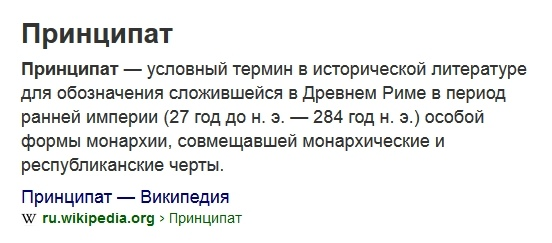
\includegraphics[scale=0.6]{Mariy/160169918019293337.png}
	%	\label{fig:scipion} % Unique label used for referencing the figure in-text\end{document}
	%	%\addcontentsline{toc}{figure}{Figure \ref{fig:placeholder}} % Uncomment to add the figure to the table of contents%----------------------------------------------------------------------------------------
	\caption{Из Вики}%	CHAPTER 2
\end{figure}

\textbf{Вывод: в четвертом разделе автор просто и незатейливо несет какую-то хуйню, не относящуюся к его тезису примерно никак. У вас принципат отклеился.
}

\section{Охуительный вывод из данной охуительной статьи}

\textit{С расширением экспансии и увеличением численности армии в Римской республике возникают процессы, которые искусственно объединяются историками в «реформу Мария». Эти процессы включают расширение класса военнообязанных римских граждан за счёт понижения планки имущественного ценза и призыва на военную службу бедняков ок. 212 и ещё раз ок. 123 гг. до н.э. Непрекращающиеся военные действия на территории провинций приводят к увеличению срока службы граждан, легионы фактически превращаются в постоянные гарнизоны, размещавшиеся на границе в готовности отразить нападение противника. Процент профессиональных солдат в их рядах непрерывно возрастает. Государство фактически берёт в свои руки функцию снабжения рекрутов оружием и военным снаряжением. Марий хотя и играл значительную роль в развитии этих процессов, сам не проводил активных реформ, способных форсировать или ослабить их ход. Потому они едва ли должны быть напрямую связаны с его именем.
}

А теперь моё заключение. Вся статья - кликбейтовое говно в стиле «МОНГОЛЬСКОГО ИГА НЕ БЫЛО», абсолютно водянистое и лишенное конкретики, тезисы подогнаны отвратительно, куча фактических ошибок, какой-то принципат у него образовался, основанный Марием арсенал не имеет к Марию отношения, половина населения Республики в армии служит и так далее. Госпаде, и в меня всерьез тыкают этой хуетой вполне неглупые люди. Вот что значит публикация в журнале, авторитетность сразу растет и публика некритически заглатывает за щеку, даже не пытаясь понять что ей затирают. Не то что эти исторические паблики, не правда ли? Но зная эту кухню, могу сказать что журнал не виноватый, да и автор тоже. Автор гонит кликбейт, не сильно вникая, томушта платят за знаки и ебись оно конем. А издание хуячит его в публикацию, томушта просмотры дает и збс. А то что за шесть лет уже целое поколение выросло с мнение что «марианская реформа то не настоящая» - это всем допизды. Ну, кроме меня, наверное, томушта это мне данный бред выслушивать приходится раз в пару месяцев, сукаблядь. Но ладно уж. 

\begin{figure}[h!tb] 
	\centering
\includegraphics[scale=0.6]{Mariy/1593599741150795821.png}
	%	\label{fig:scipion} % Unique label used for referencing the figure in-text\end{document}
	%	%\addcontentsline{toc}{figure}{Figure \ref{fig:placeholder}} % Uncomment to add the figure to the table of contents%----------------------------------------------------------------------------------------
	%	\caption{Из Вики}%	CHAPTER 2
\end{figure}

Причем автор полностью проебал такие замечательные вещи как радикальную перекройку обоза, для чего пришлось весь этот табор тупо включить в состав легиона. Ну, кузнецы, снабженцы, шлюхи, вот это вот всё. До Мария обоз был численностью до половины армии, в среднем, и крайне её замедлял. Марий решил проблему, после него римский обоз - самый маленький в античном мире, а римские легионы - самая мобильная пехота эпохи. И про то что теперь легионеры получали долю добычи минуя Сенат автор тоже не сказал ничего. Что, опять таки, полностью поменяло правила игры, и солдаты просто молились о том, чтобы началась война. Автор вообще нихуя не понимает, он высосал из пальца четыре удобных картонных тезиса, типа их «опроверг» и всё. Достаточно. Публика схавает. И публика схавала, за это респект.


Напоследок процитирую классика: «Дети, не ешьте говно, соблюдайте гигиену мозга».